\chapter{Implementation}%Jens
Due to the agile nature of the prototype development the implementation stage begun while the design phase was still underway. This chapter describes what went into the implementation of the final prototype.

\section{Micro controllers}%Daniel
	Initially doing the implementation phase, research went into what kind of micro controller, if any, we would need to construct a working prototype. Initially we settled for an Arduino Mega 2560, but going into the production phase, we realized that an external sound source was needed. The Beaglebone Black with the Bela shield suited this purpose, and was taken in during this process.
	\subsection{Arduino}%Daniel
		The Arduino is a small, but versatile micro controller, used around the world for DIY projects. The Arduino Mega, with the ATMEGA2560 chip is one of the more powerful variants, with a bigger EEPROM and more pins than the more commonly seen Arduino Uno. The pin amount was paramount in the decision to what micro controller was needed to control the physical interface, as the design called for a 4 by 5 grid of fields that should be individually activated.
		
	\subsection{Bela}%Jens
		Due to the sound related limitations from the Arduino Mega, we decided to add a connection to a Beaglebone with a Bela shield\footnote{Bela website: \url{https://bela.io/}}. The Bela provides a broad span of audio processing opportunities to create and manipulate audio as it is compatible with Pure Data(PD). PD is a visual programming language for multimedia that can also be used to create sounds.
		
	
\section{Code}
	\subsection{Arduino}%Daniel
		\begin{listing}[H]
			\caption{Example 1}
			\label{listing:example1}
			\begin{minted}[frame=lines,framesep=2mm,baselinestretch=1.1,fontsize=\footnotesize,linenos]{cpp}
struct SequenceField {
  int octave = 4;
  Field activatedFields[5];
};

struct Segment {
  bool enabled = true;
  int ledPin;
  SequenceField sequence[4];
};
			\end{minted}
		\end{listing}
		
		\begin{listing}[H]
			\caption{Example 2}
			\label{listing:example2}
			\begin{minted}[frame=lines,framesep=2mm,baselinestretch=1.1,fontsize=\footnotesize,linenos]{cpp}
void writeSegments() {
  for(int i = 0; i < amountOfSegments; i++) {
	EEPROM.put(i*sizeof(Segment), segments[i]);
  }
}
			\end{minted}
		\end{listing}
	
		\begin{listing}[H]
			\caption{Example 3}
			\label{listing:example3}
			\begin{minted}[frame=lines,framesep=2mm,baselinestretch=1.1,fontsize=\footnotesize,linenos]{cpp}
void readSegments() {
  for(int i = 0; i < amountOfSegments; i++) {
	EEPROM.get(i*sizeof(Segment), segments[i]);
  }
}
			\end{minted}
		\end{listing}
	
		\subsubsection{Libraries}%Daniel
	\subsection{PureData}%Jens
	Figure \ref{fig:pdPatch} shows the main patch of the PD code that was uploaded to the Bela. It takes inputs through the Belas' pins from the Arduino Mega. The PD patch is responsible for playing the sounds when the pads are pressed, changing the octave by multiplying/dividing the oscillators' frequencies by 2, playing the count in sound before recording or playing.
	
	\begin{figure}[H]
		\centering
		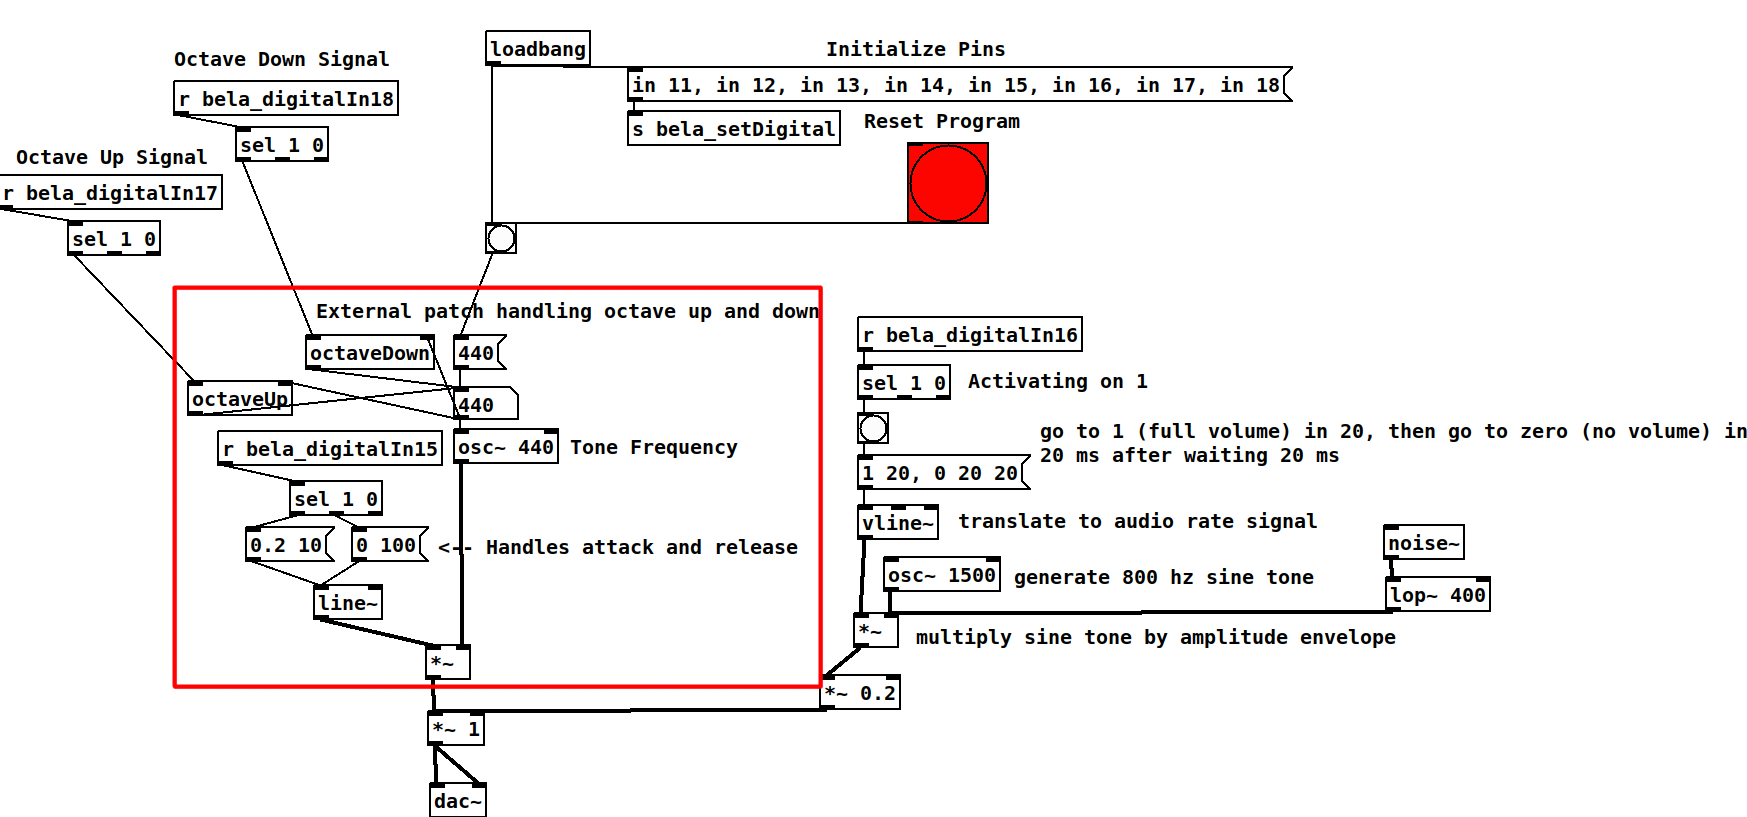
\includegraphics[width=1\linewidth]{figure/Implementation/pdPatch}
		\label{fig:pdPatch}
		\caption{Figure showing the main Pure Data patch for the prototype}
	\end{figure}	
	



\section{The box}%Jens

	\subsection{CAD}
		
	\subsection{Assembly}
	
		\begin{figure}[H]
			\centering
			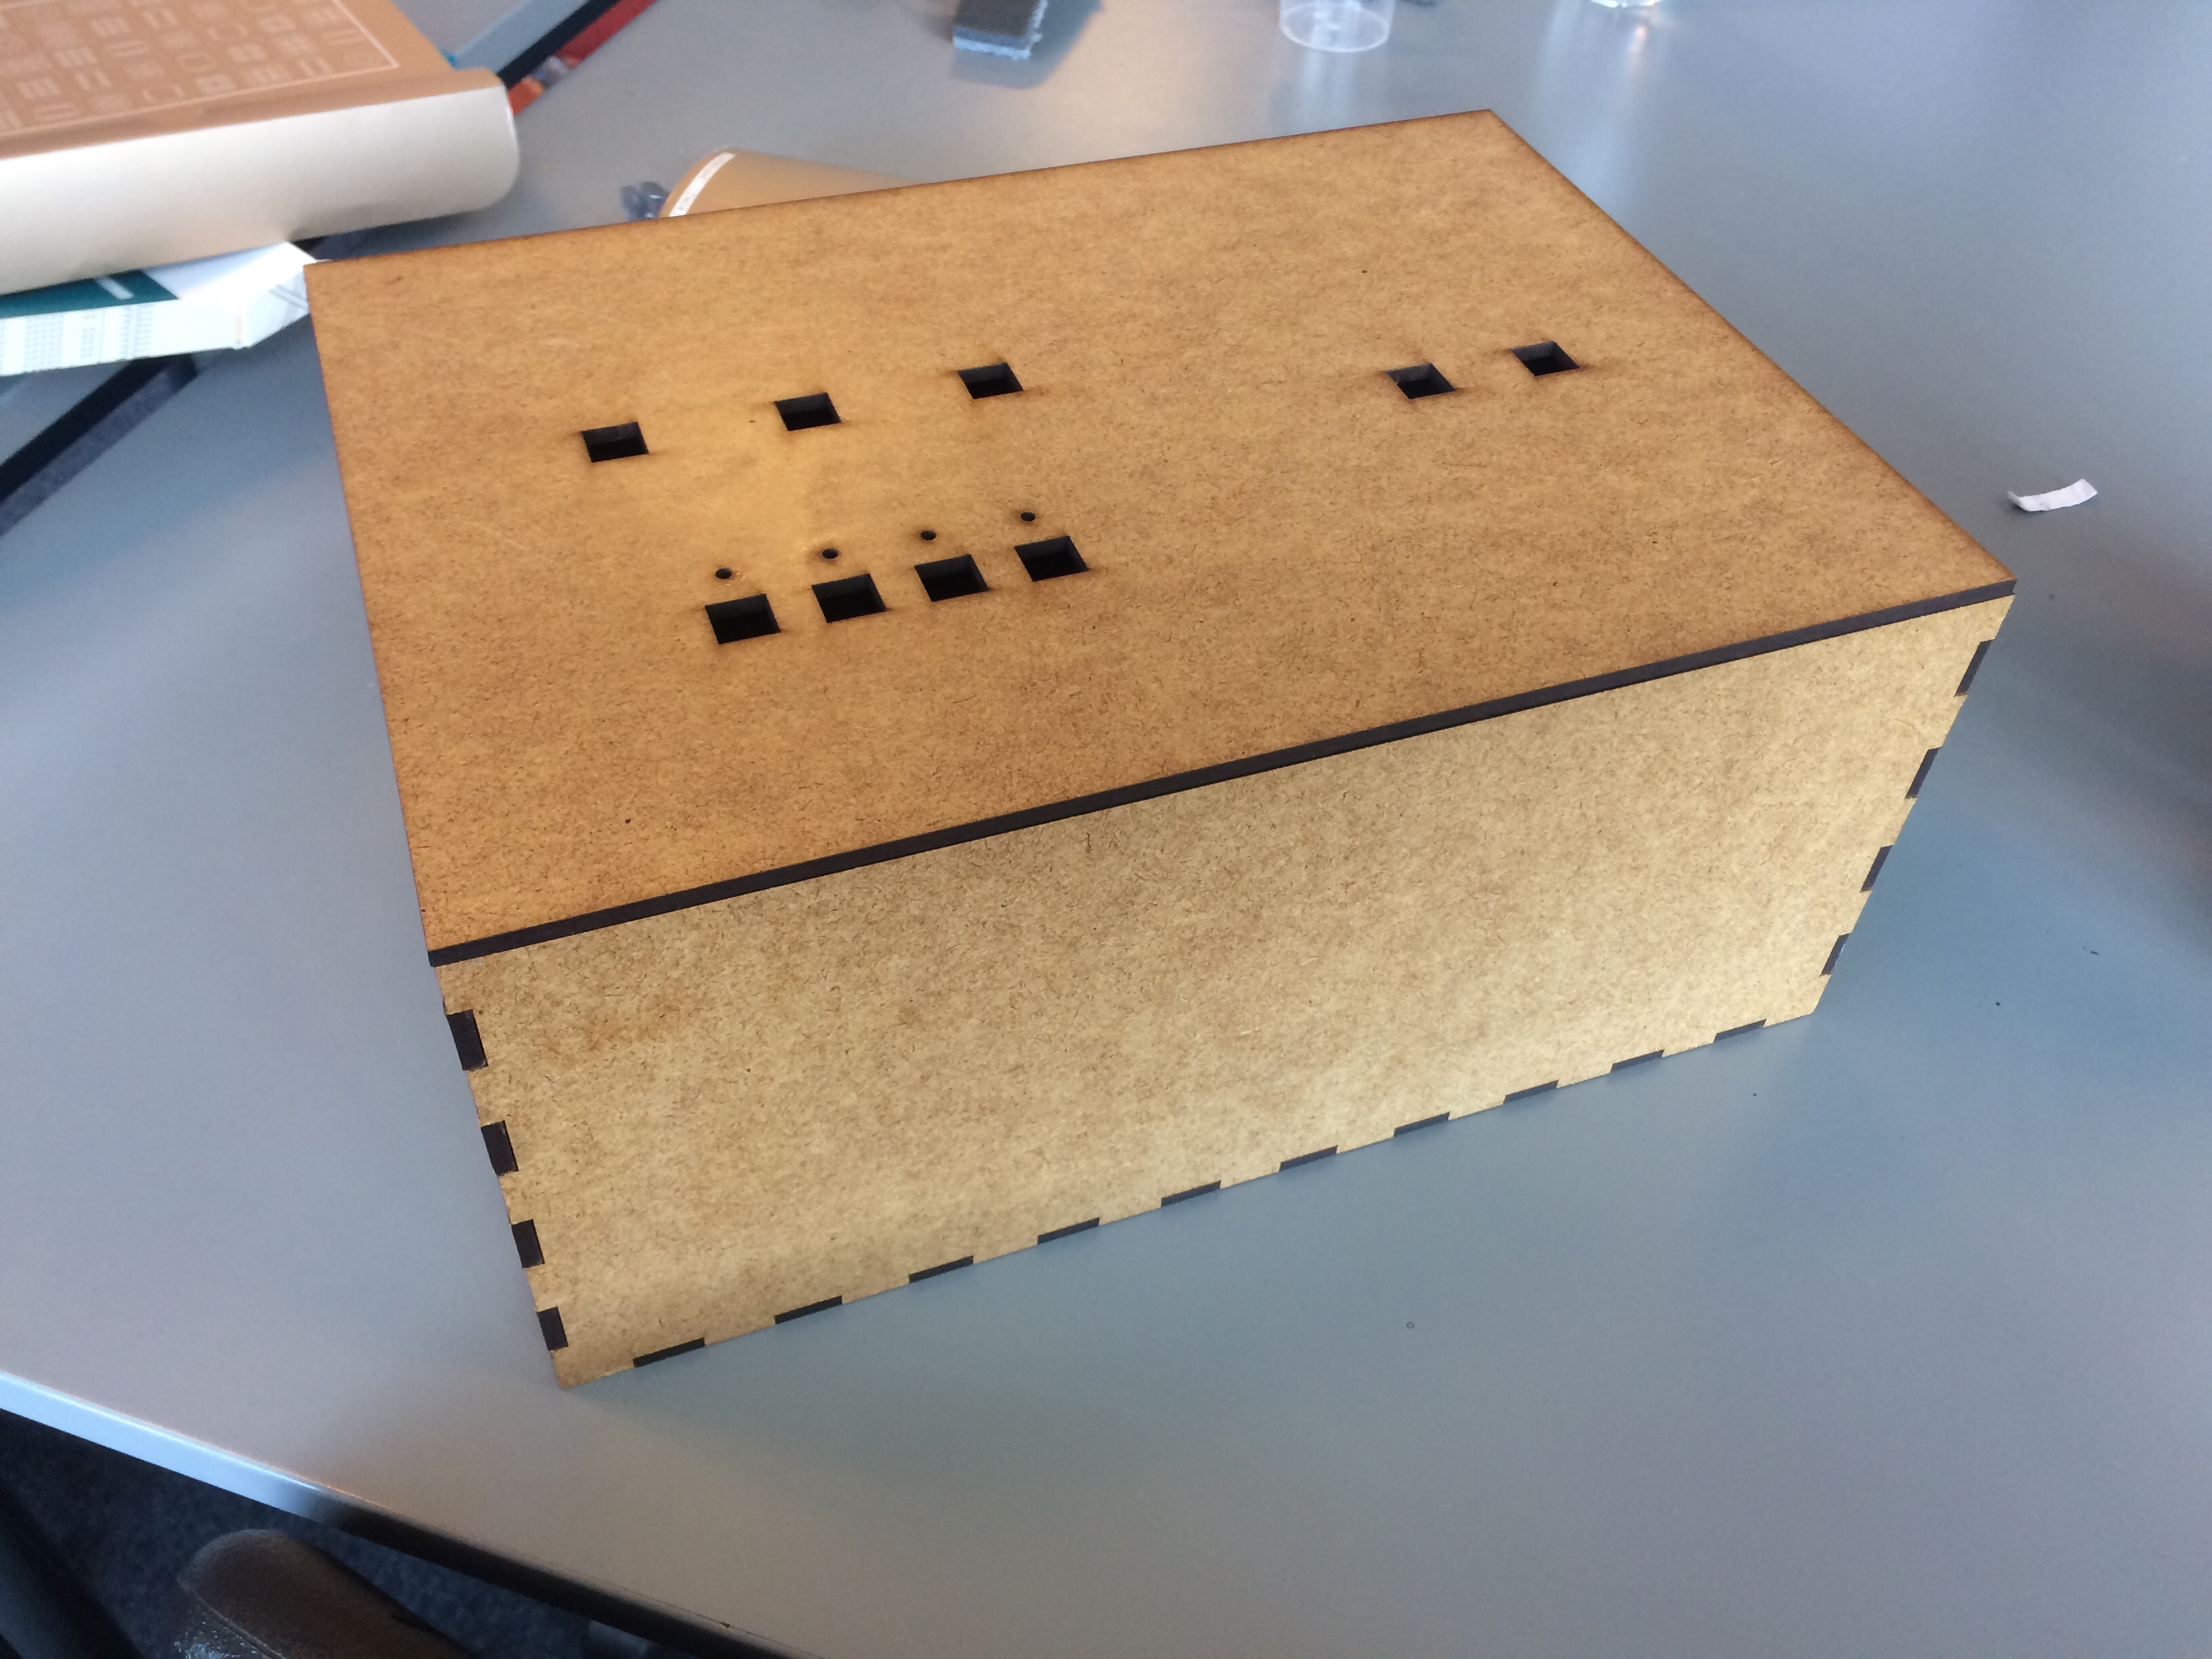
\includegraphics[width=0.7\linewidth]{figure/Design/finalbox1}
			\label{fig:finalbox1}
			\caption{The final prototype box}
			
		\end{figure}
	
		\begin{figure}[H]
			\centering
			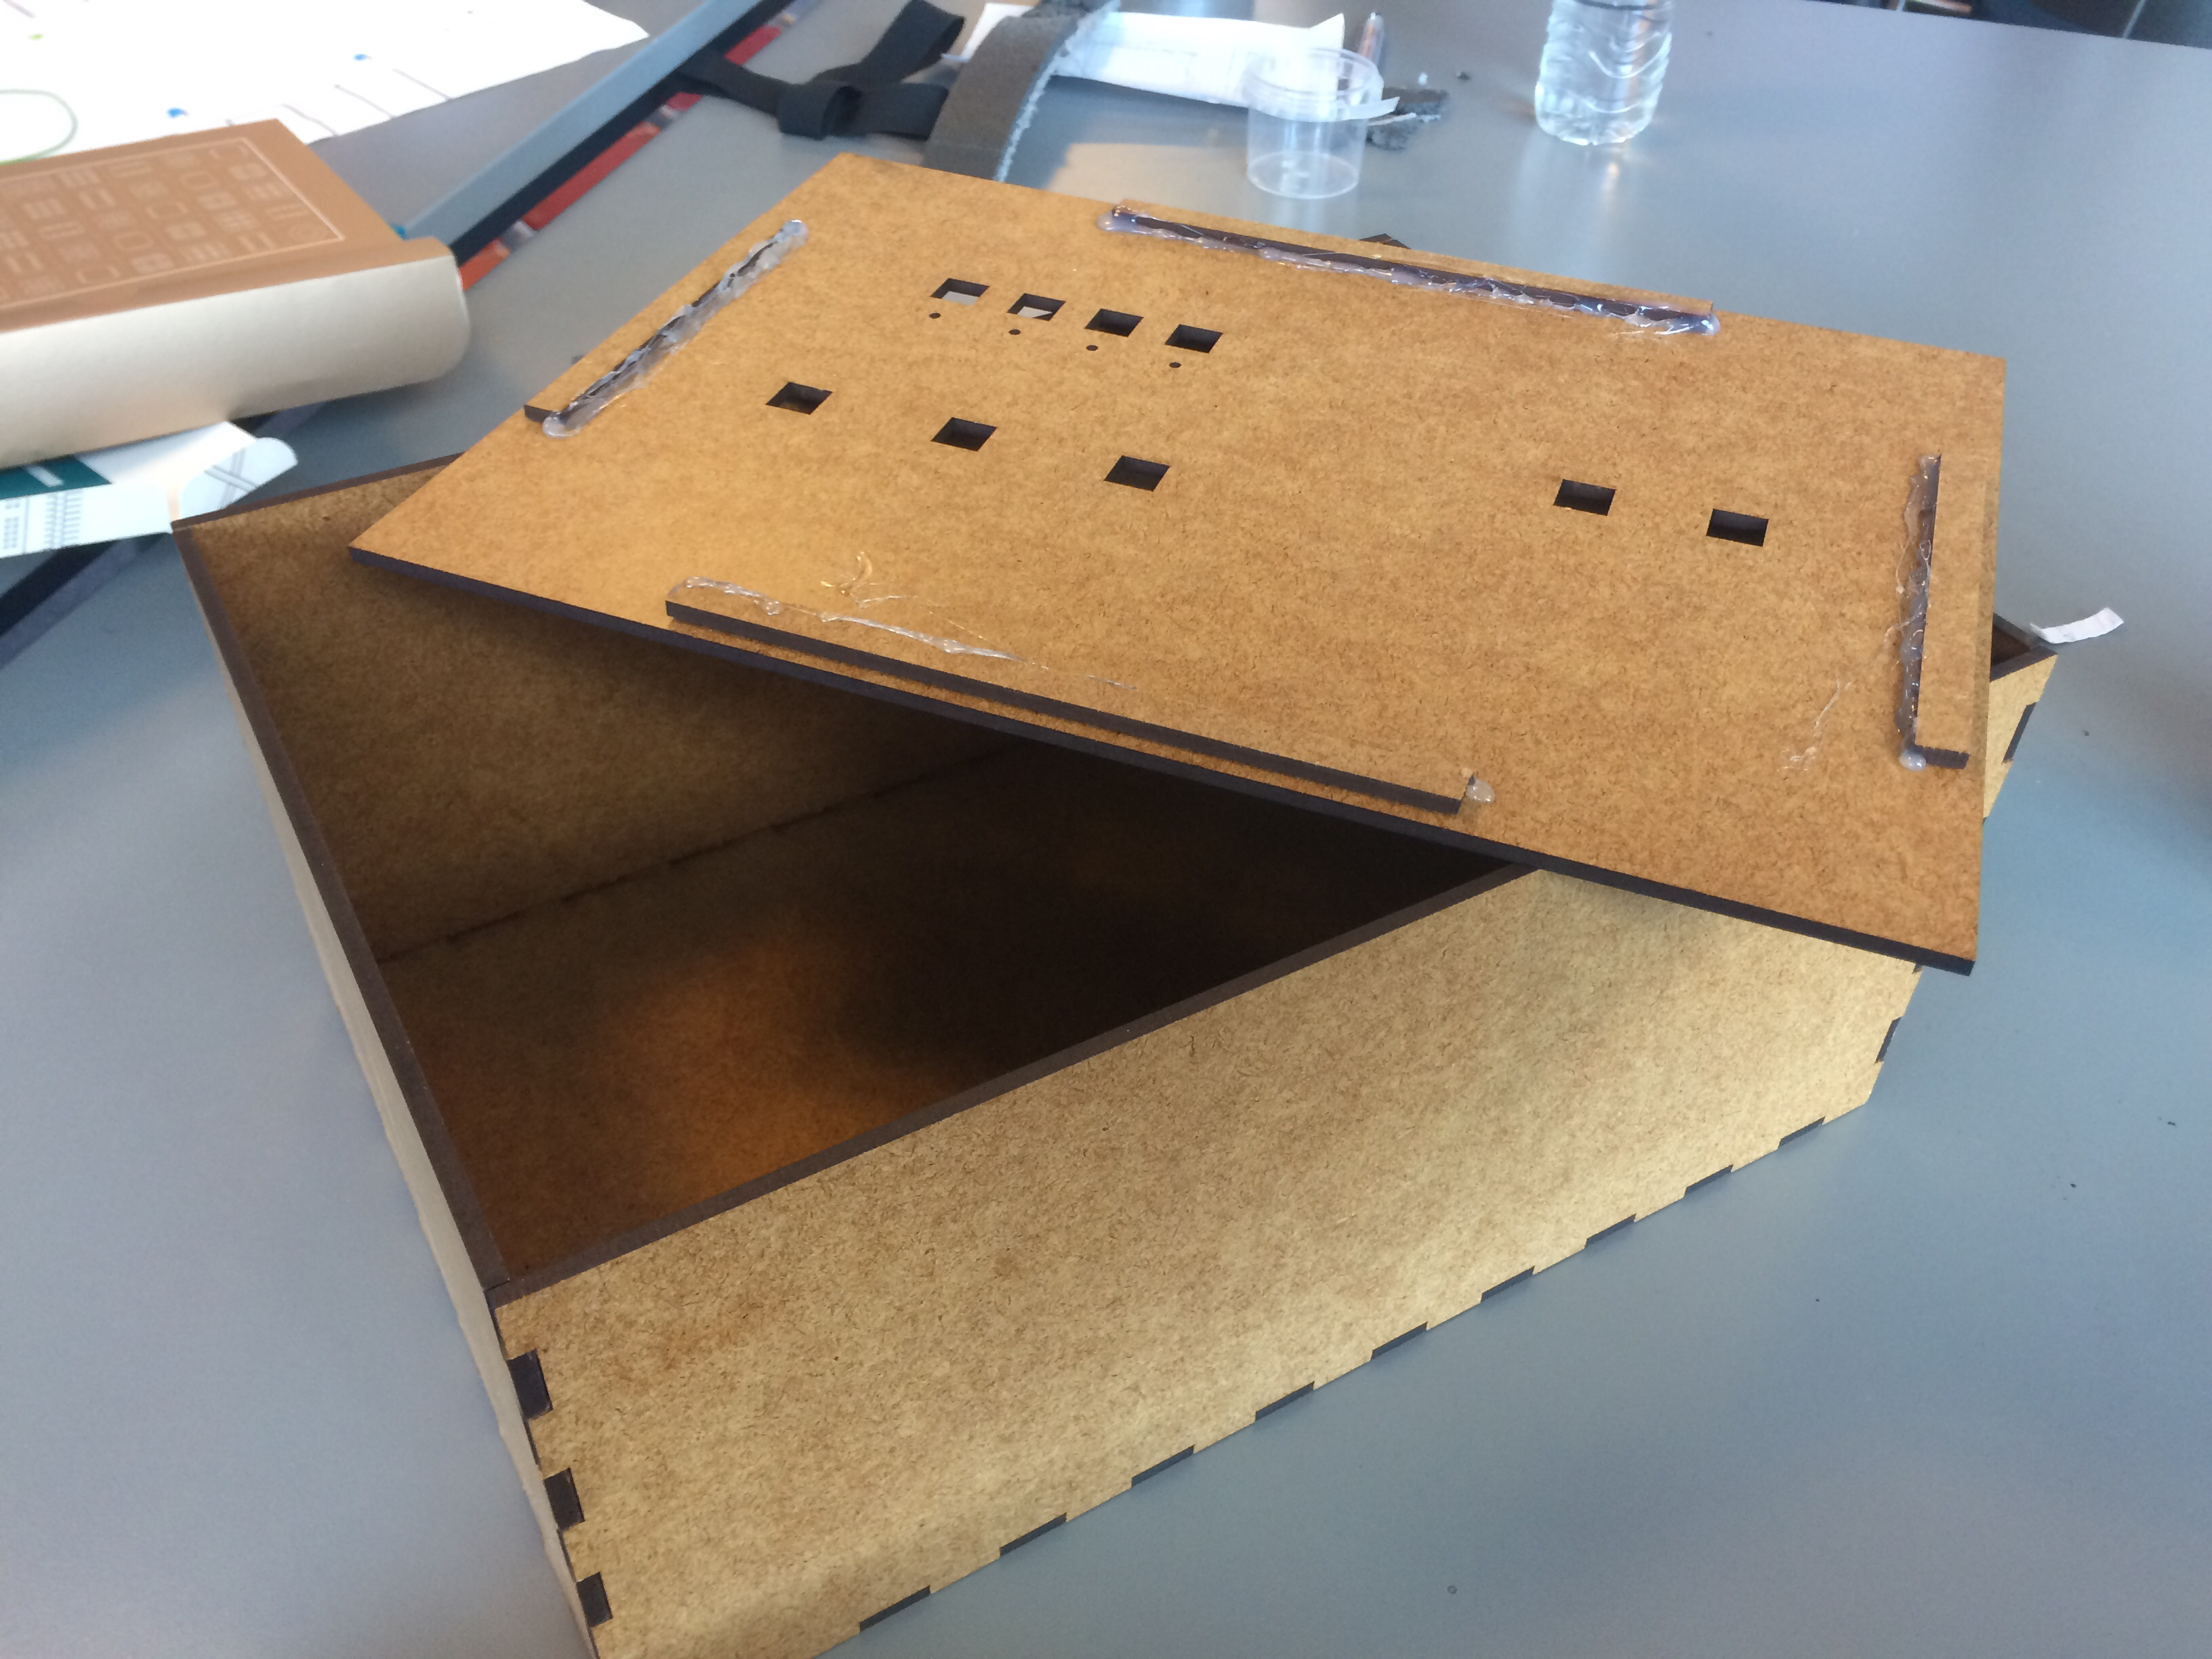
\includegraphics[width=0.7\linewidth]{figure/Design/finalbox2}
			\label{fig:finalbox2}
			\caption{The final prototype box}
		\end{figure}
		
		\begin{figure}[H]
			\centering
			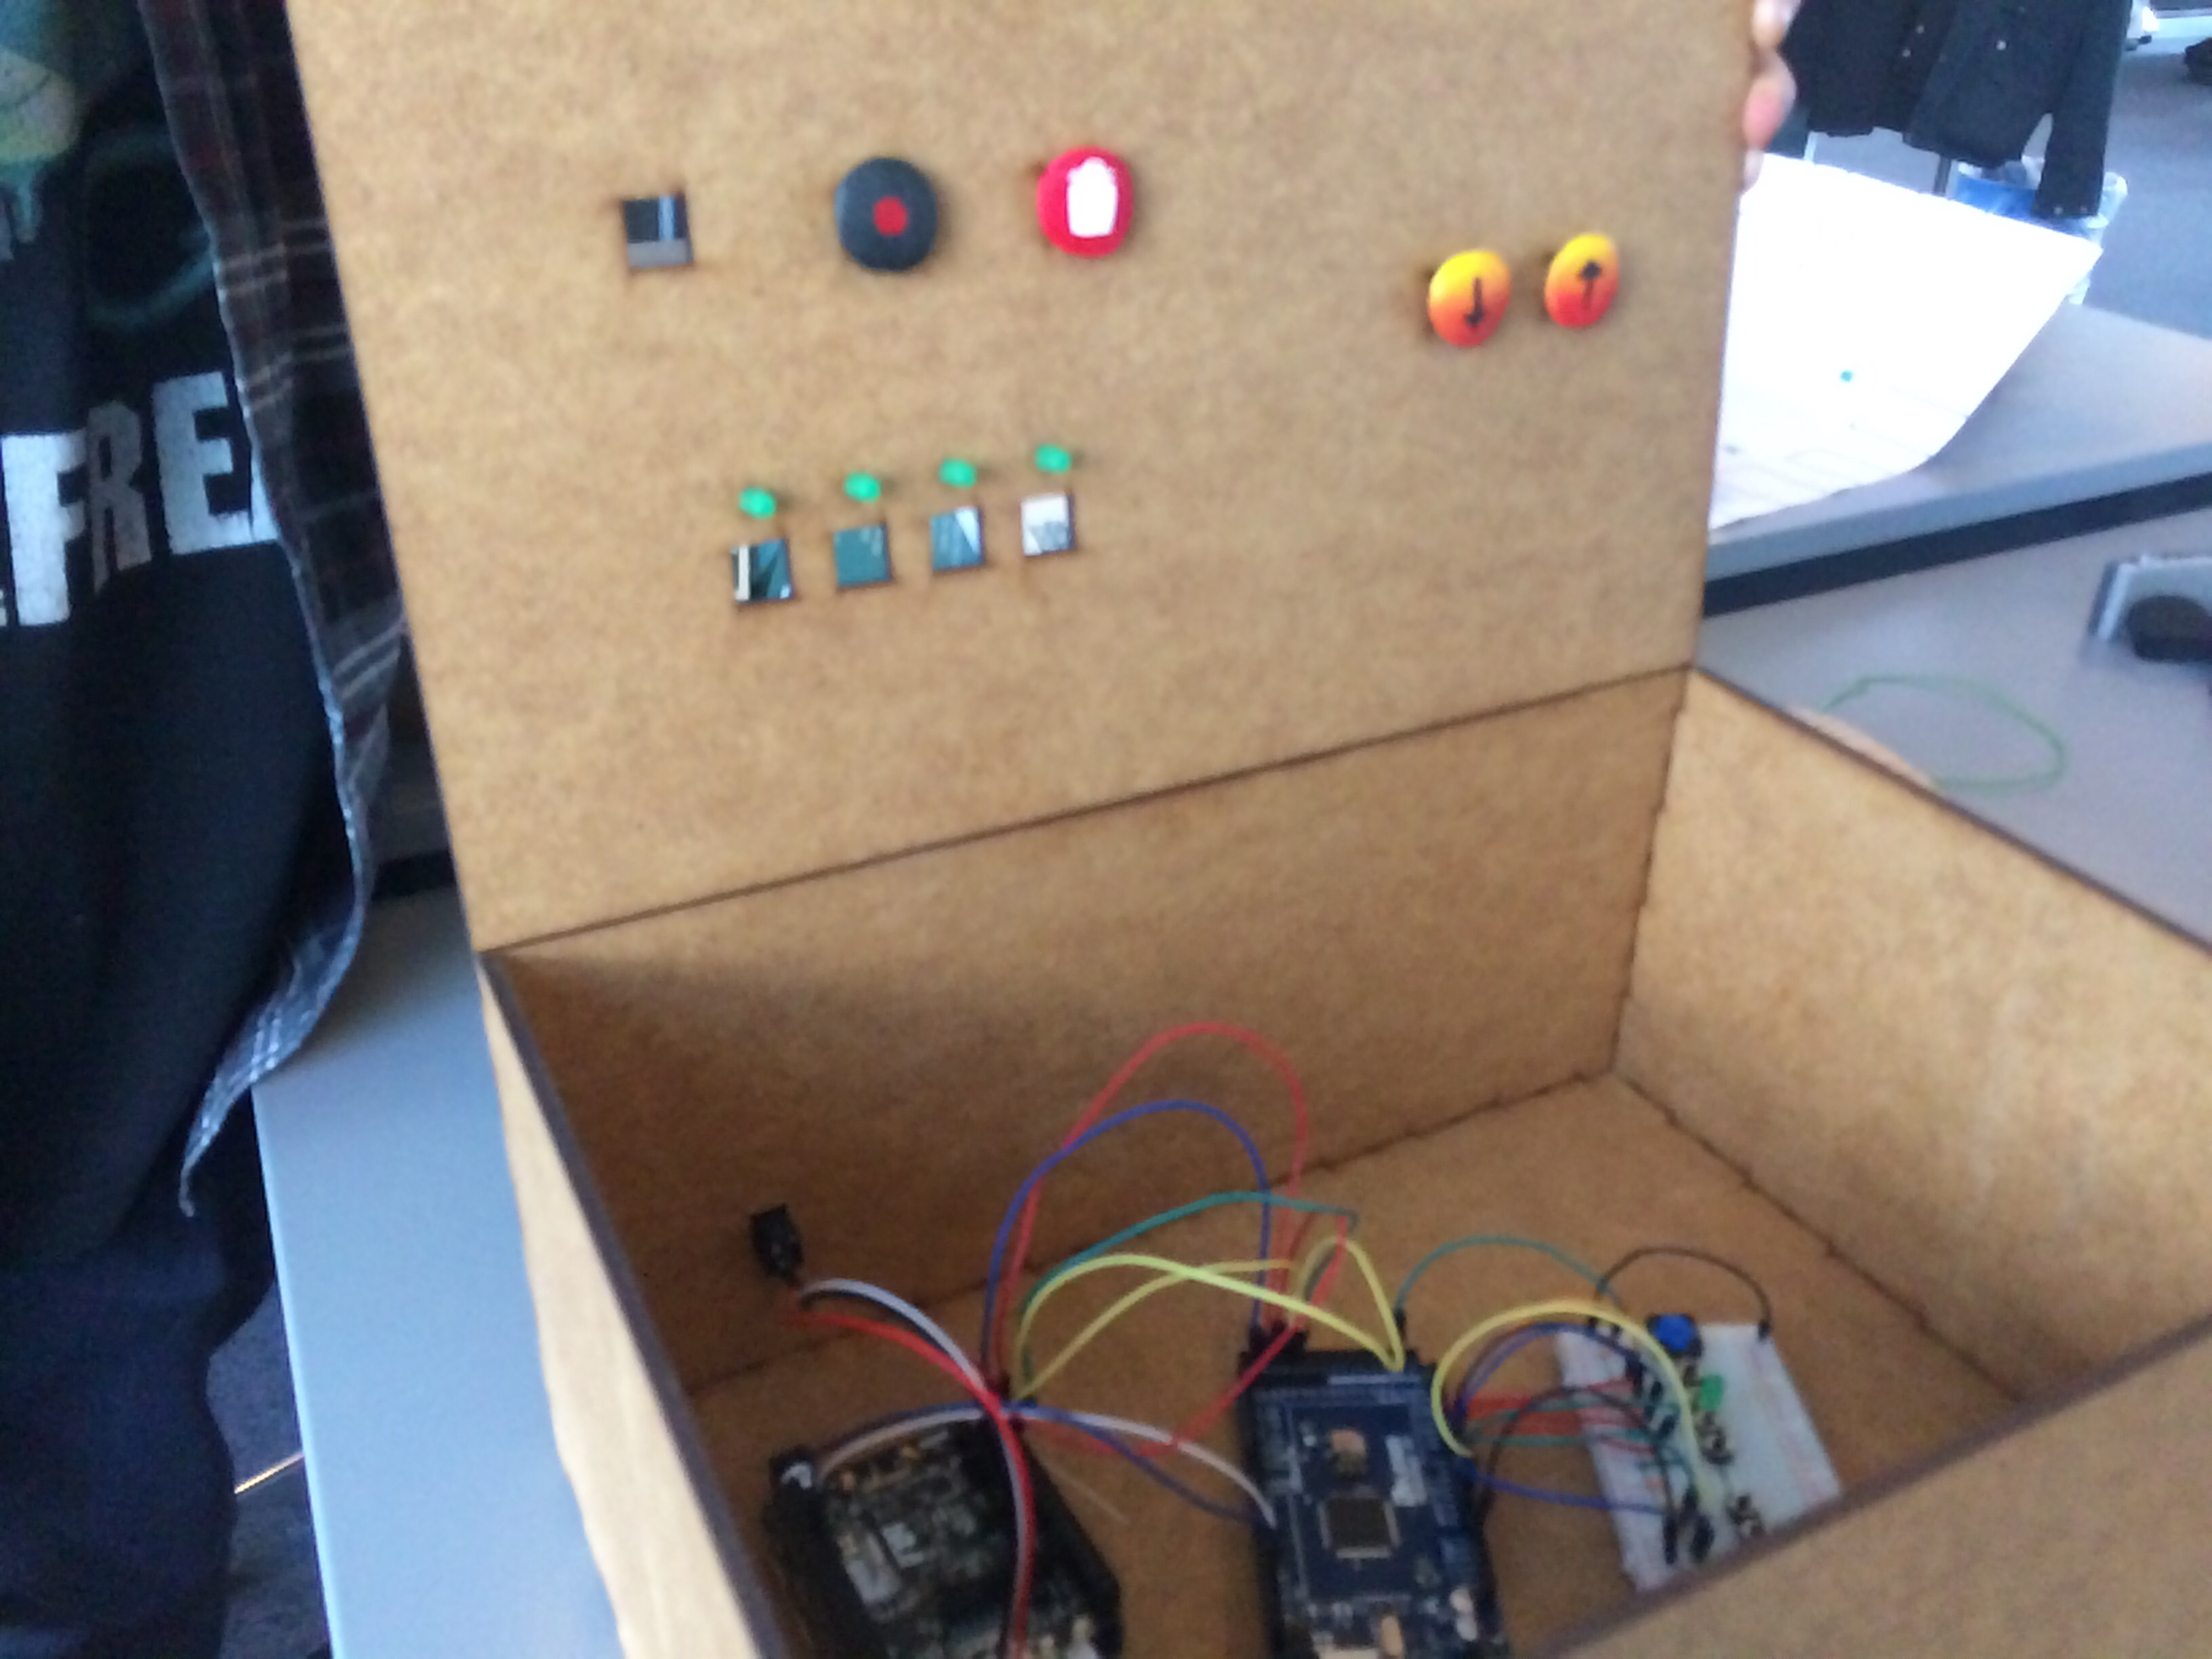
\includegraphics[width=0.7\linewidth]{figure/Design/finalbox3}
			\label{fig:finalbox3}
			\caption{The final prototype box with the electronic components inside}
			
		\end{figure}

\section{The mat}%Daniel

\section{Circuit}